\documentclass[12pt,a4paper, titlepage]{article}
\usepackage[a4paper,nomarginpar,total={170mm,257mm},left=40mm,right=25mm,top=20mm, bottom=20mm]{geometry}
\usepackage[utf8]{inputenc}
\usepackage[L7x]{fontenc}
\usepackage[lithuanian]{babel}
\usepackage{amsmath}
\usepackage{amsfonts}
\usepackage{amssymb}
\usepackage{tgtermes}
\usepackage{multirow}
\usepackage[
backend=biber,
style=apa,
url=false,
sorting=nyt
]{biblatex}
\addbibresource{bibliography.bib}


\usepackage{graphicx}
\usepackage{float}
\usepackage{setspace}
\onehalfspacing

\usepackage{hyperref}
\hypersetup{colorlinks=true,
linkcolor=black,
filecolor=blue
urlcolor=blue,
citecolor=blue}

\title{„Suaugusiųjų mokymosi problema Lietuvoje: ar nuolatinis kompetencijų kėlimas galėtų pagerinti Lietuvos ekonomiką?“}
\author{Akvilė Žiliūtė}

\begin{document}
\maketitle
\tableofcontents
\newpage

\section{Įvadas}
\subsection{Kaip apibrėžiamas suaugusiųjų mokymasis ir kam jis reikalingas?}
\paragraph{}
	ES suaugusiųjų mokymosi politika, terminą suaugusiųjų mokymasis, apibrėžia taip – „tai įvairiausia tiek bendrojo, tiek profesinio formaliojo, neformaliojo ir savaiminio mokymosi veikla, kurios imasi suaugusieji baigę pirminio švietimo ir mokymo pakopą“(\cite{bonjean_2019}). Nors pačių kompetencijų kėlimas gali būti susijęs ir su labiau buitiškomis sritimis, tokiomis kaip: deklaracijų pildymas, mokesčių formos, asmeninis tobulėjimas, kalbų mokymasis, pilietiškumo sampratos ugdymas (kodėl svarbu dalyvauti rinkimuose), melagingų naujienų atpažinimas ir t.t.
	
\begin{figure}[H]
\center
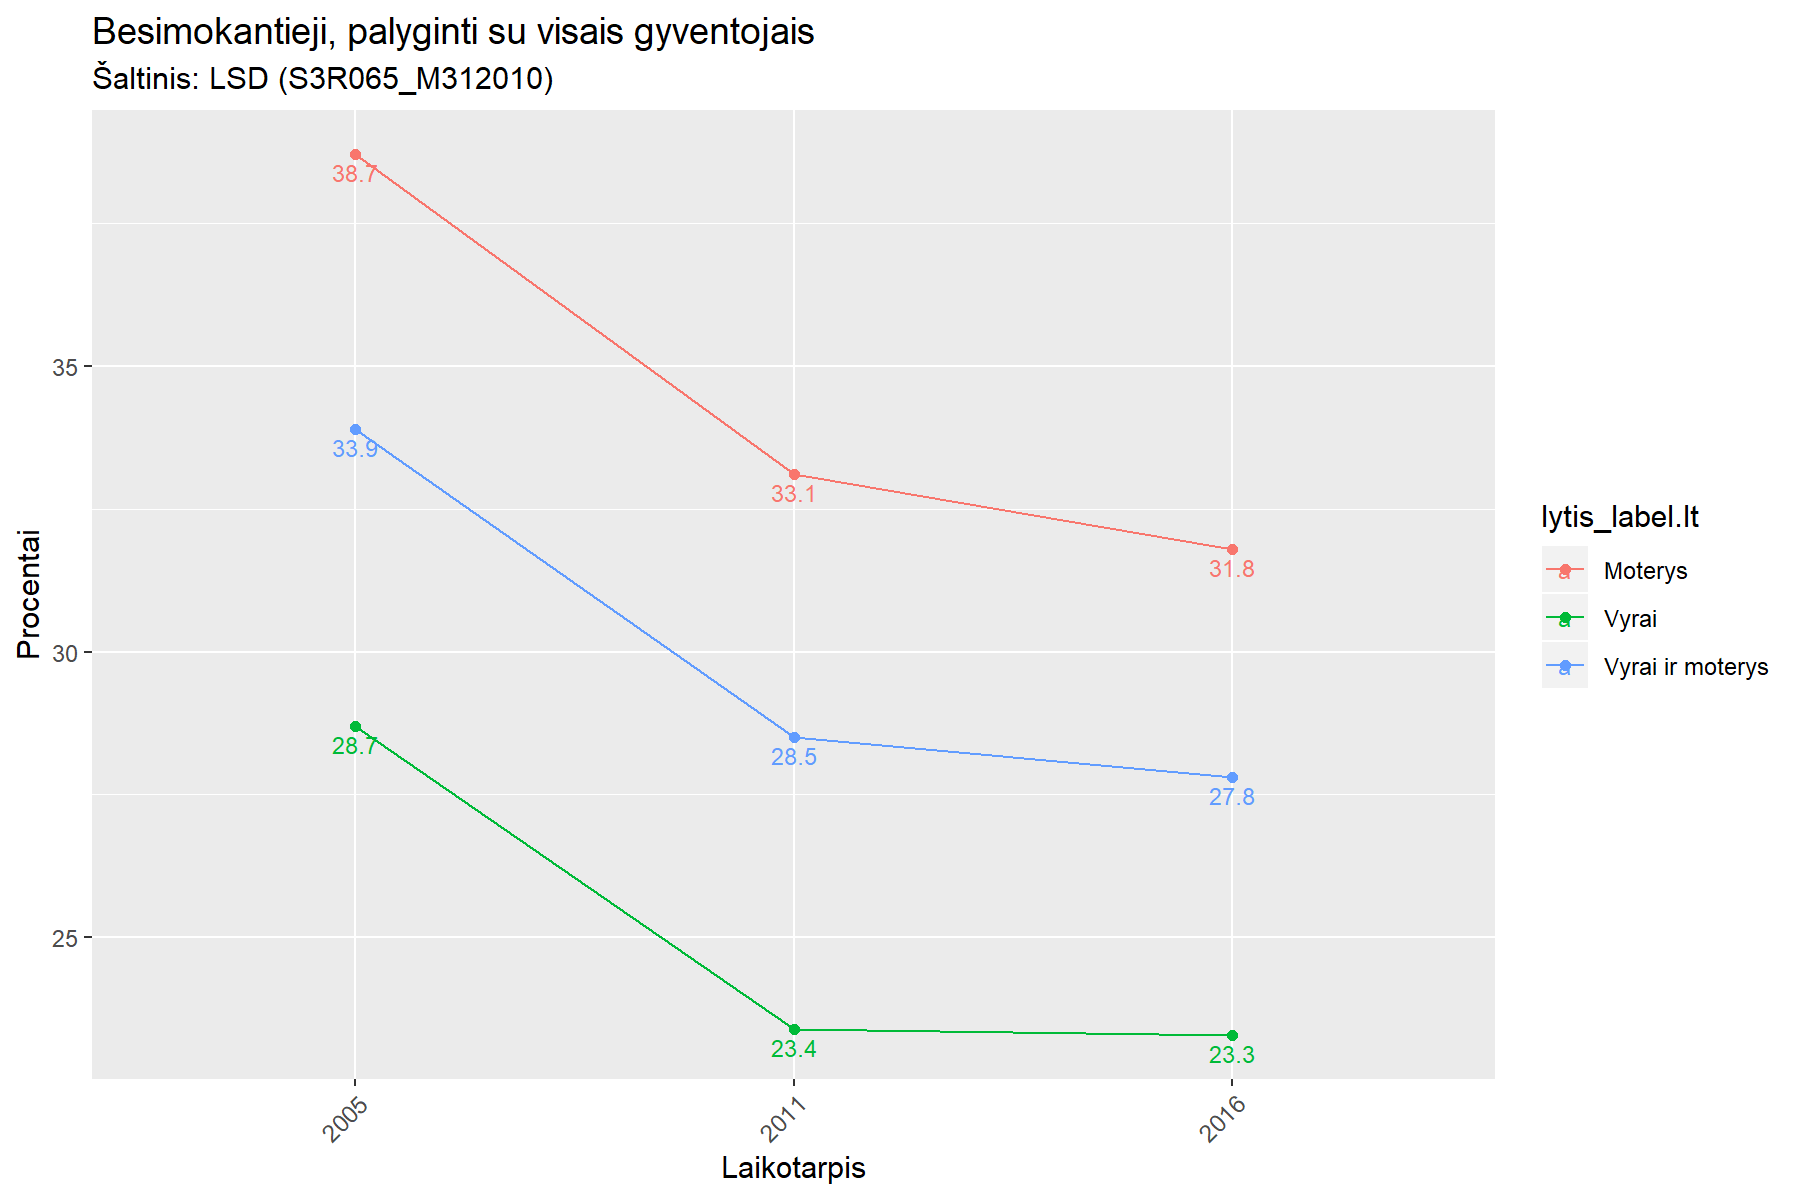
\includegraphics[scale=0.75]{Besimokantieji_palyginti_su_visais_gyventojais}
\caption{grafikas 1}
\end{figure}

\paragraph{}
	 Suaugusieji gali mokytis savo malonumui arba dėl darbe reikalingų įgūdžių. Savišvieta modernėjančiame pasaulyje tampa vis svarbesnė ir Lietuvoje matosi tendencija, jog žmonės siekia saviugdos ir ypatingai moterys yra labiau linkusios mokytis naujų dalykų, nes visuomenės požiūris į moterį keičiasi, dabar moterys dažniau nori siekti karjeros, o ne tik būti namų šeimininkėmis.  Tad viso gyvenimo mokymasis gali būti raktas į naują gyvenimo etapą ir karjeros pradžia. Pagal grafiką matome, kad 2005 m. visų gyventojų net 38,7 proc. moterų užsiėmė formaliu arba neformaliu švietimu, tiesa vėliau tendencija mažėjanti ir 2016 m. liko tik 31,8 proc. visų respondentų. Tuo tarpu vyrų, kurie 2005 m. užsiėmė formaliu arba neformaliu švietimu, buvo tik 28,7 proc., 2016m. tendencija taip pat sumažėjo iki 23,3 proc. Iš viso paskutiniais Lietuvos statistikos dapartamento duomenimis, Lietuvoje 2016m. formaliu arba neformaliu švietimu užsiėmė 27,8 proc. visų gyvenojų. Vėliau tai paanalizuosime Europos kontekste.  
\paragraph{}
	  Analizuojant Klaipėdos universiteto dėstytojos Julijos Melnikovos tyrimą „Kokybiško mokyklų vadovų kompetencijų ugdymo komponentų projektavimas suaugusiųjų švietimo paslaugų optimizavimo kontekste“, galima pastebėti, kad žmonių dirbančių su vaikais ir mokytojais asmeninis tobulėjimas yra vienas iš svarbiausių veiksnių šiuolaikinėje švietimo sistemoje. Tyrime aprašoma mokyklos vadovų kompetencijų kėlimo projektavimas, eiga ir refleksijos. Analizuojant tyrimo rezultatus bei refleksijas, pastebėtina, kad vadovai, kurie dalyvavo šiame projekte, mokėsi ne tik su dėstomu kursu susijusių naujovių ar bendradarbiavimo su mokytojais principų, bet nagrinėjo lyderystės aspektus, komunikacijos svarbą, gilinosi į savo pačių vidines asmenybes siekdami pagerinti savo, kaip mokytojų ir vadovų, bendravimą su mokiniais ir kitais mokyklos darbuotojais.  Refleksijose vadovai džiaugėsi, jog turėjo galimybę pažinti save ir suprasti, kad mokymasis yra nesibaigiantis gyvenimo procesas. Šis tyrimas tik dar kartą patvirtina, kad asmeninis tobulėjimas yra ne tik profesinis žingsnis, bet ir raktas į savianalizę, savęs pažinimą (\cite{melnikova2012kokybivsko}).
\paragraph{}
 		Siekiant integruotis į Europos Sąjungą bei pasiekti aukštą šios bendrijos pragyvenimo lygį, vienas svarbiausių klausimų Lietuvoje yra suaugusiųjų mokymosi problemos iškėlimas.  Ši problema yra sukonkretizuota  visam Europos regionui strategijoje „Europa 2020“ bei Lietuvos valstybės pažangos strategijoje „Lietuva 2030“, kurioje „ Europos Sąjunga ir Lietuva įsipareigoja suaugusiųjų švietimui:

\begin{enumerate}

\item Kurti darnias mokymosi visą gyvenimą sistemas;
\item Užtikrinti lengvesnį perėjimą iš vieno švietimo lygmens į kitą;
\item Didinti suaugusiųjų mokymosi prieinamumą ir galimybių mokytis įvairovę;
\item Gerinti suaugusiųjų švietimo kokybę;
\item Skatinti visuomenės pilietiškumą;
\item Formuoti teigiamas suaugusiųjų nuostatas apie mokymosi visą gyvenimą svarbą ir naudą;
\item Plėtoti įvairiais būdais įgytų kompetencijų pripažnimą.“ (\cite{Zablacke2015}).

\end{enumerate}

\section{Suaugusiųjų mokymasis Lietuvoje}

\subsection{Suaugusiųjų mokymosi Lietuvoje vertinimas ir progresas Europos kontekste}
\paragraph{}

\begin{figure}[H]
\center
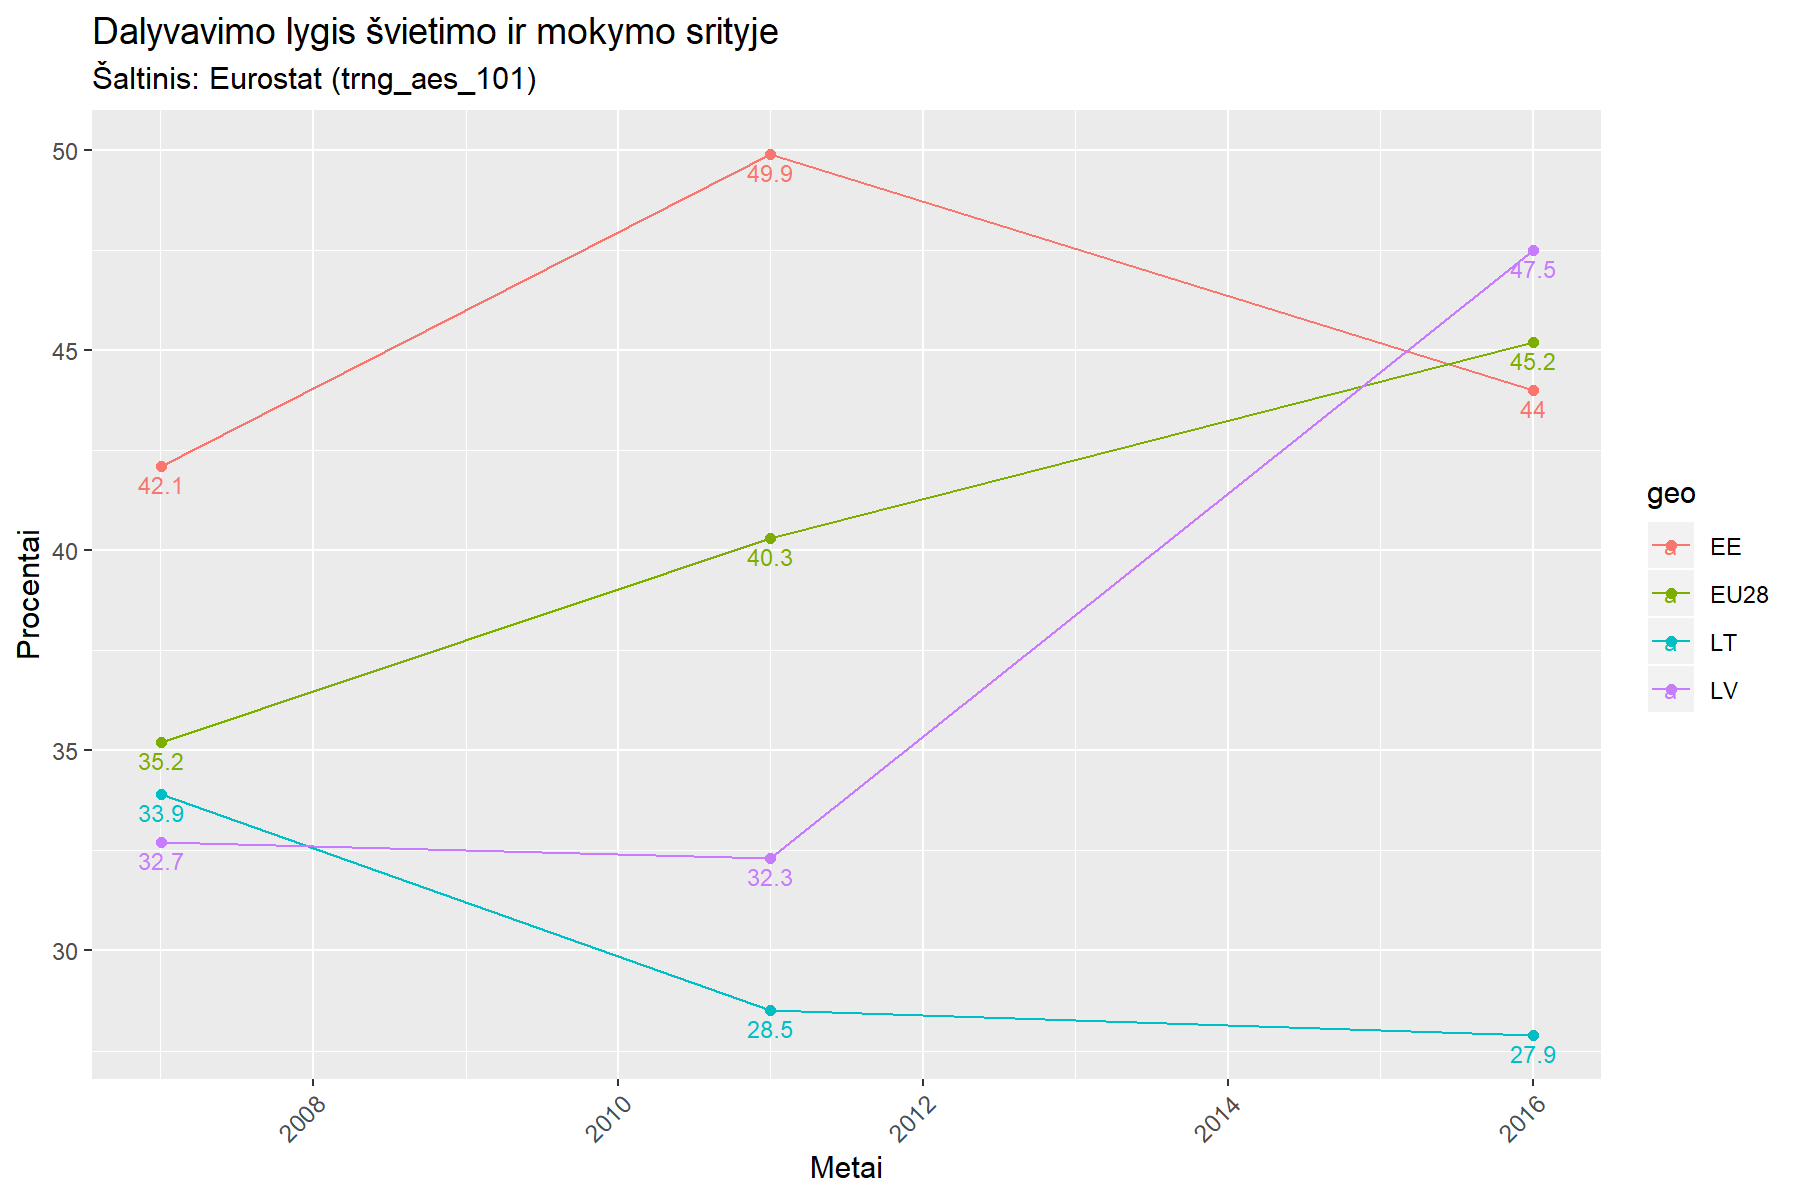
\includegraphics[scale=0.75]{Dalyvavimo_lygis_svietimo_ir_mokymo_srityje}
\caption{grafikas 2}
\end{figure}

Pagal grafiko duomenis matome, jog nuo pat 2008 m. suaugusiųjų mokymosi rodikliai Lietuvoje visada buvo žemesni ne tik už Europos Sąjungos vidurkį, bet ir gerokai žemesni už kitų Baltijos šalių rodiklius. Mažiausias skirtumas buvo 2007 m. Lietuvoje tuomet jis siekė 33,9 proc., o Europos Sąjungos rodiklis buvo 42,1 proc. Iki 2011 m. Europos Sąjungos tendencija progresyviai didėjo ir 2011 m. pasiekė 49,9 proc., tuo tarpu Lietuvoje rodiklis buvo 28,5 proc. Na ir 2016 m. Europos Sąjungos rodiklis šiek tiek sumažėjo ir buvo 44 proc., o Lietuvos vis toliau žemėjo ir paskutiniais duomenimis turime, jog 2016 m. dalyvavusių švietimo ir mokymo srityje tėra tik 27,9 proc. nuo visų gyventojų. Kalbant apie suaugusiųjų mokymosi Lietuvoje ir Europos Sąjungoje palyginimą, atsiveria akivaizdūs skirtumai, tačiau tie skirtumai atsiranda dėl skirtingų tradicijų ir istorinio konteksto. Europoje gerokai anksčiu buvo pradėta skatinti žmones tobulėti, stengtis pažinti save, mokytis naujų dalykų ne tik dėl darbo reikalavimų, bet ir dėl bendrųjų kompetencijų kėlimo. Lietuvoje situacija šiek tiek kitokia, mūsų savianalizės tradicijos gerokai skiriasi, nes istoriškai ne visada Lietuva buvo laisva šalis ir negalėjome formuoti visuomenės mentaliteto gręžiantis tik į Vakarų Europą. Totalitarinio rėžimo valdymo metu lietuviai net nedrįsdavo galvoti apie Europos šalių kalbų mokymasi, viso gyvenimo mokymosi programą, elementarių naujų technologijų pritaikomumo galimybes. Tad kolkas mes vis tik siekiame ir lygiuojames į Europos Sąjungos suaugusiųjų mokymosi rodiklius.
\paragraph{}	
	 Prof., habil dr.M.Teresevičienės,  dr. V.Zuzevičiūtės, R.Kuncaičio, A.Rutkienės tyrimo “Suaugusiųjų mokymasis Lietuvoje: aprėptis, poreikiai ir pasiūla” ataskaitoje atsispindi būtent saugusiųjų mokymosi vizija, kurią įgyvendinę mes būtumėme dideliu žingsniu arčiau Europos Sąjungos: „Lietuvos dokumentuose, sudarytuose pagal Europos Sąjungos 16 reikalavimus, išryškėja tendencija, skatinti suaugusius žmones savo problemas spręsti per mokymąsi, tobulėjimą. Teigiama, jog svarbu suaugusiuosius išmokyti mokytis, vėl pajusti, kad pažinimas ar nuolatinis domėjimasis savo ir visuomenės gyvenimu atgaivina asmeninį žmogaus budrumą, leidžia jam realizuoti save, savo sumanymus ir taip padėti sau ir valstybei vystytis. Šių poreikių tenkinimą užtikrina neformalusis suaugusiųjų švietimas.“(\cite{teresevivciene2006tyrimo}). Šiame tyrime buvo nagrinėjama Suaugusiųjų mokymosi situacija Lietuvoje, atsižvelgdami į tyrimo išvadas galime teigti: „Lietuvoje yra sukurta neformalųjį švietimą reguliuojanti įstatymine bazė bei parengti strateginiai sistemos plėtros dokumentai, kurie atitinka Europos Komisijos direktyvas bei Mokymosi visą gyvenimą memorandume suformuluotas nuostatas“; oficialumo ir formalumų Lietuvoje trūkumas  padaro suaugusiųjų mokymasi nepatraukliu ir neturinčiu tęstinumo; „nepriklausomai nuo gyvenamosios vietos, amžiaus ar lyties – didžiausias poreikis yra užsienio kalbų mokymuisi“; pagrindinė žmonių nesimokymo ir nesidomėjimo svarbais dalykais priežastis yra lėšų trūkumas, paprastai Lietuvoje žmonės visą savo laiką skiria papildomų lėšų uždirbimui, gyvenimo kokybės gerinimui; informacijos apie suaugusiųjų mokymosi galimybes tyrimo dalyviai paprastai gauna iš darboviečių, žiniasklaidos, tad tai yra akivaizdus komunikacijos trūkumas, siekiant išplėsti susidomėjimą viso gyvenimo mokymosi programa (\cite{teresevivciene2006tyrimo}).
\paragraph{}	 
	  Koncentruojantis  į 2018m. Europos komisijos vertinimą suaugusiųjų mokymosi aspektu, ten teigiama:
\begin{itemize}
\item „Šalis padarė nedidelę pažangą gerindama švietimo ir mokymo sistemos, įskaitant suaugusiųjų mokymąsi, kokybę, veiksmingumą ir atitiktį darbo rinkos poreikiams.“
\item Europos komisijos rekomendacijos: „Gerinti švietimo ir mokymo sistemos, įskaitant suaugusiųjų mokymąsi, kokybę, veiksmingumą ir atitiktį darbo rinkos poreikiams.“ (\cite{Rekomendacija2018}).
\end{itemize}



\subsection{Suaugusiųjų mokymosi Lietuvoje ypatumai ir galimybės}
\paragraph{}
	Kadangi kolkas suaugusiųjų mokymasis Lietuvoje yra vis dar labai nepopuliarus, tad šios veiklos ypatybės nėra išskirtinės. Kaip teigiama Švietimo ir mokslo ministerijos problemos analizėje „Suaugusiųjų mokymasis: kiek mokosi, ką moka, ar turi galimybių mokytis?“, viso gyevnimo mokymosi programa domisi aukštesnės kvalifikacijos specialistai, nes jie supranta kompetncijų kėlimo svarbą ir naudą, o žemesnio išsilavinimo žmonėms paprastai trūksta kompetencijų, reikalingų prieš pradedant mokymosi programą, ar net ieškant informacijos apie suaugusiųjų mokymosi galimybes Lietuvoje. Analizėje apibrėžiamos aštuonios svarbiausios reikalingos kompetencijos, reikalingos kiekvino žmogaus asmeniniam tobulėjimui: „tai kalbos, raštingumo, mokėjimo skaičiuoti ir informacinių komunikacinių technologijų (IKT) įgūdžiai, o visos ugdymo(si) veiklos yra grindžiamos mokėjimu mokytis. <...>Tokie gebėjimai kaip kritinis mąstymas, kūrybingumas, iniciatyvumas, problemų sprendimas, pavojaus įvertinimas, sprendimų priėmimas ir konstruktyvus jausmų valdymas atlieka pagrindinį vaidmenį ugdant visas aštuonias kompetencijas.“ (\cite{Zablacke2015}).

\begin{figure}[H]
\begin{tabular}{ |l|l| } 
\hline
Kompetencijų grupės & Gebėjimai  \\
\hline
\multirow{3}{8em}{Kalbų mokėjimas} & Bendravimas gimtąja kalba \\ 
& Bendravimas užsienio kalba \\ 
\hline
\multirow{3}{10em}{Informaciniai gebėjimai} & Matematiniai, mokslo ir
technologijų gebėjimai \\ 
& Skaitmeninis
raštingumas  \\ 
\hline
\multirow{3}{12em}{Visuomeniniai ir socialiniai įgūdžiai} & Kultūrinis sąmoningumas ir raiška \\ 
& Mokymasis mokytis\\ 
& Socialiniai ir
pilietiniai
gebėjimai\\
& Iniciatyvumas ir
verslumas\\
\hline
\multirow{3}{12em}{Bendrosios kompetencijos} & Kritinis mąstymas \\ 
& Kūrybingumas\\ 
&Iniciatyvumas\\
&Problemų sprendimas\\
&Konstruktyvus jausmų valdymas\\
&Pavojaus įvertinimas\\
&Sprendimų priėmimas\\
\hline
\end{tabular}
\caption{lentelė 1}
\end{figure}



	Lentelės duomenimis matome, kad kompetencijas galime  suskirstyti grupėmis, tad pradėdami naują mokymosi programą, reikėtų įsivertinti, kur turime daugiauiai žinių, o kur dar reikėtų tobulėti. Taigi galima daryti išvadą, kad norint išmokti naujų dalykų turi būti motyvuotas ir gebėti naudotis savo jau turimomis žiniomis ir gebėjimais. 
\paragraph{}		
	Labai dažnai naujų dalykų mokymasis ilgalaikiams bedarbiams suteikia didelius šansus susirasti mėgiamą darbą bei pažinti savo norus. Žvelgiant iš kitos pusės, kaip teigia Vilniaus Gedimino technikos universiteto dėstytoja Laima Okunevičiūtė-Neverauskienė bei darbo ir socialinių tyrimų instituto atstovas Arūnas Pocius staripsnyje „Ilgalaikio nedarbo problema Lietuvoje“, ilgalaikius bedarbius būtų galima suskirstyti į keturias grupes: „1) 25 proc. ypač aktyvūs (pasirengę ir kelti kvalifikaciją (persikvalifikuoti), ir laikinai įsidarbinti). 2) 12 proc. orientuoti tik į profesinį tobulėjimą, bet nepasirengę dirbti viešųjų (laikinųjų) darbų. 3) 54 proc. pasirengę dirbti tik viešuoius (laikinuosius) darbus, bet nepasiruošę tobulėti profesiniu požiūriu. 4) 9 proc. ypač pasyvūs (nepasirengę dalyvauti aktyviose priemonėse arba abejojantys)“ (\cite{pocius2003ilgalaikio}). Taigi šis suskirstymas atskleidžia dar vieną svarbų suaugusiųjų mokymosi Lietuvoje ypatumą – gyventojų pasyvumą. Net tie, kurie didžiąją gyvenimo dalį yra praleidę be darbo ir net neturi jokių garantijų oriai senatvei užsitarnauti visai nėra pasiruošę kelti savo kvalifikacijos, iš viso 63 proc. ilgalaikių bedarbių nesuvokia išsilavinimo ir viso gyvenimo mokymosi svarbumo ir iš čia iškyla visuomeninė problema, kad galbūt viso gyvenimo mokymosi programa nėra tinkamai iškomunikuota ir ištransliuota žmonėms, nes kalbant apie šį dalyką būtina paminėti svarbą ne tik dėl darbo reikalų, bet ir visos Lietuvos ateities, nes kompetetingi ir motyvuoti žmonės kuria gerokai didesnę pridedamąją vertę visuomenės gerovei.
\paragraph{}	
	 Dar vienas suaugusiųjų mokymosi ypatumas, kaip išskyrė Mykolo Riomerio universiteto dėstytoja Dr. Rita Aleknaitė-Bieliauskienė straipsnyje „Lietuvos suaugusiųjų ugdymo sistemos ypatumai“ – „Suaugusiųjų mokymas susietas su darbo rinkos problemomis.“ (\cite{aleknaite2014lietuvos}). Čia taip pat minima, kad didžiausią darbo pasiūlos dalį sudaro arbo pasiūlymai mokantiems naudotis kompiuterinėmis technologijomis, mokantiems programuoti. Tad natūralu, kad šioje srityje suaugusieji dažniausiai ir nori pagilinti savo žinias.
\paragraph{}	 

\begin{figure}[H]
\center
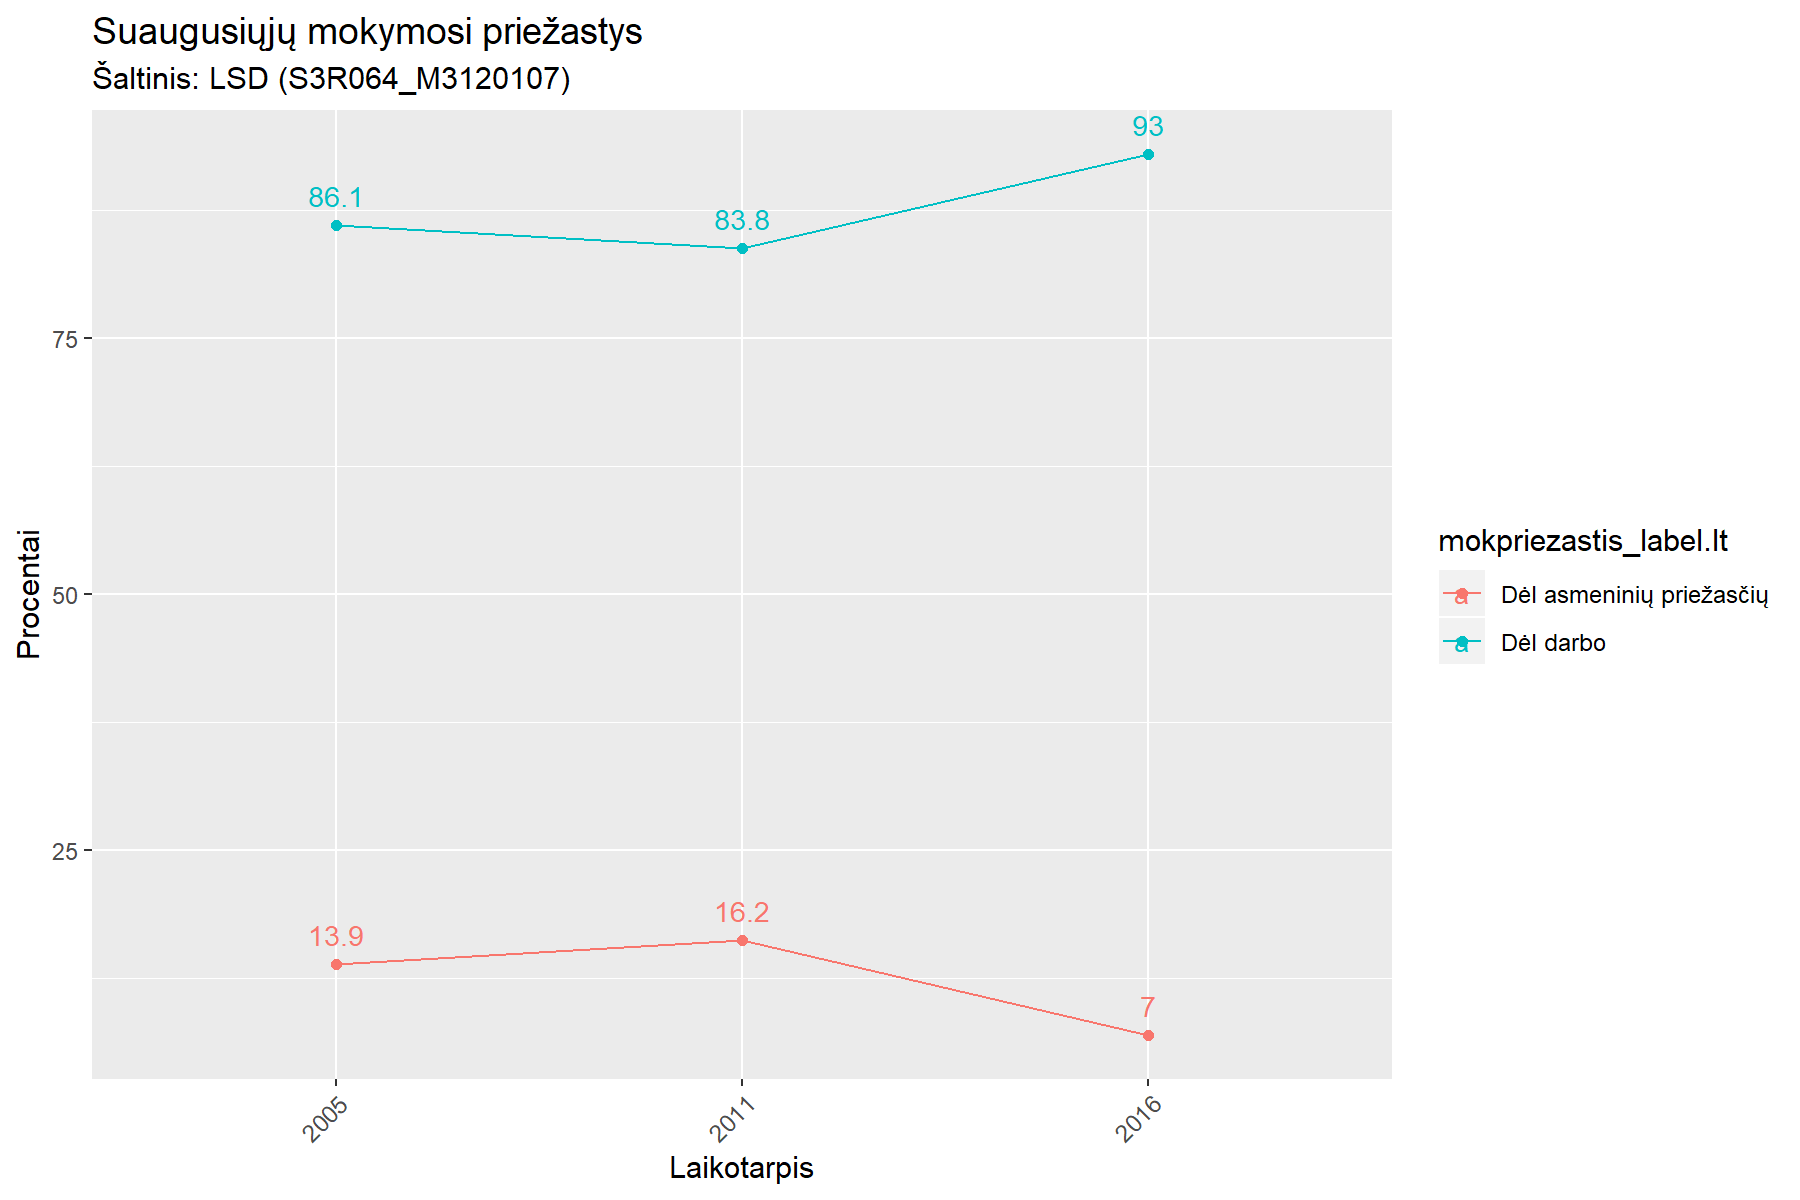
\includegraphics[scale=0.75]{Suaugusiuju_mokymosi_priezastys}
\caption{grafikas 3}
\end{figure}

	   Paskutinis ypatumas, kurį norėčiau pabėžti, tai, kad priežastys, kodėl žmonės mokosi ir kaip jie mokosi skiriasi nuo kiekvieno žmogaus charakterio savybių, lietuviai paprastai yra pasyvūs žmonės, todėl čia dažniausiai suaugusieji mokosi tik tada, kai to reikalauja darbas ar priėmimo į darbą sąlygos. Kaip rodo grafikas, 2016 m. duomenimis 93 proc. besimokančių suaugusiųjų kėlė savo kompetencijas dėl darbo ir tik 7 proc. dėl asmeninių poreikių. Tai yra pagrindinis rodiklis, parodantis, kad lietuviai nėra suinteresuoti pažinti save bei mokytis visą gyvenimą, jie tai daro tik skatinami būtinųjų aplinkybių. Kitose Europos valstybėse į mokymąsi yra žiūrima kaip į kasdienybę, todėl ten žmonės mokosi naujų dalykų kasdien, jiems tai yra įprasta ir reikalinga. 
\paragraph{}
	Konkrečiai diskutuojant apie pačias mokymosi visą gyvenimą galimybes Lietuvoje, tai visų pirma, reikėtų pabrėžti, kad šis mokymasis yra skirstomas į formalų („Lietuvos suaugusieji pagal formaliojo švietimo programas gali mokytis kelių tipų įstaigose: bendrojo lavinimo mokyklose, suaugusiųjų švietimo centruose, profesinėse mokyklose, kolegijose ir universitetuose. Šios įstaigos, išskyrus bendrojo lavinimo mokyklas, rengia kvalifikacijos tobulinimo ir perkvalifikavimo kursus, kurie taip pat sudaro dalį suaugusiųjų švietimo“, - Europos suaugusiųjų mokymosi elektroninė platforma (\cite{shpitzer_2019}) ir neformalų („Neformalųjį suaugusiųjų švietimą gali vykdyti neformaliojo suaugusiųjų švietimo įstaigos, suaugusiųjų mokymo centrai, aukštosios mokyklos, kvalifikacijos tobulinimo institucijos, įmonės, nevyriausybinės organizacijos, asmenys ir kt. Suaugusiųjų mokymasis vyksta darbo vietoje, jį, atsižvelgdami į verslo poreikius, organizuoja darbdaviai“,- Europos suaugusiųjų mokymosi elektroninė platforma (\cite{shpitzer_2019}).  Pagal Švietimo ir mokslo ministerijos problemos analizę „Suaugusiųjų mokymasis: kiek mokosi, ką moka, ar turi galimybių mokytis?“ išskiriamos šios, suaugusiųjų mokymosi Lietuvoje, galimybės: 
\begin{itemize}

\item EPALE (Europos suaugiųjų mokymosi elektroninė platforma) – tai platforma skirta dalintis aktualia suaugusiųjų mokymuisi informacija, renginiais,  naujienomis, pranešimais, mokymosi ištekliais, rekomendacijomis, čia atviros galimybės pradėti projektus bei užmegzti profesinius santykius. Ši platforma atvira visai Europai ir yra daugiakalbė. 
\item SMIS (Suaugusiųjų mokymosi elektroninė sistema)- tai intraktyvi nuotolinio suaugusiųjų mokymosi paslauga, kurios pagalba daug didesnė visuomenės dalis gali naudotis šia platrofma ir nuotoliniu būdu ir kiekvienam tinkamu laiku turėti neformaliojo švietimo ir tęstinio mokymosi paslaugas. 
\item UDC (universalieji daugiafunkciai centrai) – ši alternatyva sprendžia didžiųjų miestų ir mažesnių miestelių atskirtį, nes šie centrai pagrinde yra statomi kaimų vietovėse. Švietimo, kultūros, socialinės, sveikatos, sporto, užimtumo paslaugas teikiantys centrai prisideda ir prie suaugusiųjų mokymosi prieinamumo gerinimo, nes būtent čia vyksta paskaitos, seminarai ir susitikimai, kurie skatina savęs pažinimą ir viso gyvenimo mokymosi programą. 
\item TAU (trečiojo amžiaus universitetas)- „veikla, kurių paskirtis suaugusiųjų švietimo sistemoje yra apibrėžta Neformaliojo suaugusiųjų švietimo ir tęstinio mokymosi įstatyme. TAU – savarankiška, savanoriška organizacija, savo veikla užtikrinanti vyresnio amžiaus žmonių geresnę socialinę integraciją į visuomenę, skatinanti jų efektyvų, produktyvų ir turiningą gyvenimą, palaikant jų darbingumą, fizinį aktyvumą.“
\item Aukštosios mokyklos (46 aukštosios mokyklos, iš jų 19 privačios aukštosios mokyklos) – čia siūlomos aukštojo mokslo programos, bet šalia jų žmonės gali rinktis ir tikslines, susiaurintas, konkrečios disciplinos programas. Dažnai kursai ir mokymai organizuojama atsižvelgiant į norinčiųjų mokytis kiekį bei poreikius. 
\item Profesinio mokymo įstaigos (90 profesinių mokymo įstaigų, iš jų 12 privačios) – čis kuriamos sąlygos sąlygos ne tik mokytis naujų dalykų, bet ir kelti kvalifikacijos laipsnį. Taip pat viso gyvenimo mokymosi programas čia renkasi ne tik dirbatieji, bet ir bedarbiai, tai gali būti vienas iš prioritetų ieškant naujo darbo. 
\item Bibliotekos, archyvai, kitos kultūros įstaigos – ši alternatyva yra skirta motyvuotiems žmonėms, kurie netik įžvelgia mokymosi svarbumą, bet kasdien siekia pažinti save, savo poreikius ir nebijo iššūkių. Būtent ši sritis yra kelias svajonių link, nes kai žmogus pradeda mėgti skaityti knygas, jam atsiveria gerokai daugiau kelių nei prieš tai (\cite{Zablacke2015}).
\end{itemize}


\section{Suaugusiųjų mokymosi ir ekonomikos ryšys}

\subsection{Kaip suaugusiųjų mokymasis yra susijęs su ekonomika?}
\paragraph{}
	Akivaizdus klausimas, kuris kyla besiruošiantiems pradėti mokymosi programą, ar  viso gyvenimo mokymasis yra naudingas tik pačiam asmeniui? Atsakymas – tai tik visos didelės naudos dalis. Suaugusiųjų mokymosi populiarumas padidintų ne tik žmonių kompetencijų lygį, bet ir savimonės sampratą, pilietiškumą, valstybinį išsilavinimo lygį, dėl šių priežasčių suaugusiųjų mokymasis yra glaudžiai susijęs su valstybės ekonomika, nes ekonomika yra susijusi su žmonių savimone, išsilavinimo lygiu,užimtumu. Kuo žmonės yra labiau motvuoti mokytis naujų dalykų, išrasti naujoves, kurti valstybei pridedamąją vertę, tuo valstybės ekonomika turi didesnį pagrindą tapti stabilesne.
	 Remiantis ES suaugusiųjų mokymosi politika, apibendrinant suaugusiųjų mokymosi ir ekonomikos sąsajas, būtų galima išskirti šiuos aspektus: 

\begin{enumerate}

\item Aktyvesnis suaugusiųjų mokymasis gali padėti Europai įveikti ekonomikos problemas, turėti pakankamai reikiamų naujų įgūdžių įgijusių darbuotojų ir pasirūpinti, kad senėjanti jos darbo jėga išliktų produktyvi. 
\item Keldami savo kompetencijas suaugusieji turėtų gebėti suprasti kaip svarbu yra balsuoti bei šita tendencija išsirinkti valdžios atstovus, kurie mąsto kritiškai, o ne tik dalina politinius pažadus.
\item Mokydamiesi naujų, rinkos geidžiamų naujovių suaugusiesiams turėtų būti lengviau įsidarbinti ir taip būtų mažinamas nedarbas Lietuvoje.
\item Mokydamiesi visą gyvenimą žmonės didintų savo kompetencijas bei gebėtų atlikti ne tik fizinį darbą emigracijoje, tačiau kurti ir savo produktą ar turėti labiau kompetetingą darbą tėvynėje, sumažėtų emigracja (\cite{bonjean_2019}).

\end{enumerate}


\subsection{Ar suaugusiųjų mokymasis galėtų darti tiesioginę įtaką Lietuvos valstybės ekonomikos gerinimui?}
\paragraph{}
	Pastebėjus glaudžius ryšius tarp suaugusiųjų mokymosi ir ekonomikos, akivaizdu, kad bendruomeniškai siekiant pagerinti Lietuvos ekonomikos lygį, žmonės turėtų būti motyvuoti mokytis naujų dalykų, kelti savo kompetencijas bei kvalifikaciją taip kurdami didesnę pridėtinę vertę Lituvos valstybei, mažindami nedarbą, neišprūsimą, emigraciją.
\paragraph{}	
	  Užimtumo veiksnių tyrime „Užimtumą lemiančių mikroekonominių ir makroekonominių veiksnių modelis“ KTU lektorė Sandra Jakštienė būtent ir išskyrė, kad užimtumą lemia viena siš mikroekonominių veiksnių tai technikos ir technologijų ištekliai: „Technikos ir technologijų veiksniai. Ši veiksnių grupė siejama ir su asmenimis, ir su įmone ir apima inovacinei veiklai skiriamus žmogiškuosius išteklius, kurie susiję su technologiniais pokyčiais, t. y. naujovėmis, mokslo ir technikos žinių panaudojimu, dalyvavimu mokslinių tyrimų ir eksperimentinės plėtros veikloje (naujų žinių gavyba).“ (\cite{jakvstiene2013uvzimtumka}). Taigi tai patvirtina aspektą, jog asmeninis tobulėjimas ir žinių gavyba gerina ne tik asmeninį gyvenimą, bet ir valstybiniu mastu didina užimtumą. 
\paragraph{}	  
	  Kaip teigiama kitame tyrime „Suaugusiųjų mokymo(si) organizavimo ypatumai, ieškant efektyviausio sprendimo taikant ir plėtojant suaugusiųjų mokymo organizavimą“ - „Technologiniai, ekonominiai, socialiniai, inovacijų ir politiniai pokyčiai, lydimi naujų profesijų atsiradimo ir senų išnykimo, sąlygoja naują požiūrį į mokymąsi, kompetencijų bei įgūdžių ugdymą(si). Suaugusiųjų mokymasis yra svarbus ekonominis variklis.“ (\cite{kvieskiene2016suaugusikujku}). Tad minėti globalūs visuomenės veiksniai yra pagrindinis atsakymas į klausimą, kodėl svarbu plėtoti, kalbėti ir skatinti suaugusiuosius domėtis viso gyvenimo mokymosi programomis. Žmonės turi būti suinteresuoti ne tik dėl asmeninių poreikių, bet ir bendrais visuomenės tikslais, tai galėtų tapti „domino efektu“, kai žmonės varžytųsi ne dėl savo finansinių galimybių, bet išsilavinimo aspektu. „Norint paversti Lietuvą nuolat augančia, žiniomis grįsta ekonomika, didinančią darbo vietų skaičių bei gerinančią socialinius ryšius šalimi, reikia pakankamą dėmesį skirti suaugusių mokymui(si) pasitelkiant inovatyvius mokymosi metodus.“ (\cite{kvieskiene2016suaugusikujku}).
\paragraph{}	  
	   Apibendrinant šį aspektą, visuomenė turi suprasti, jog ne tik politikai yra atsakingi už mūsų praeitį, dabartį ir ateitį, o mes, patys žmonės, turime skirti pakankamai dėmesio savo išsilavinimui, kilimu karjeros laiptais, savianalizei bei asmeninių poreikių nusistatymui.
	   
\newpage
\section{Išvados}
\paragraph{}
\begin{enumerate}
\item Norint lygiuotis su kitomis Europos Sąjungos valstybėmis, bei pasiekti ES susidomėjimo  dėl mokymosi visą gyvenimą lygį Lietuva privalo ne tik plėsti mokymosi prieinamumą, tačiau ir stengtis sudominti visuomenę, įdiegti suvokimą, jog tik keldami savo kompetencijas ir domėdamiesi supančia mus aplinka, galima ne tik pagilinti senas žinias, bet ir išmokti naujų, darbus lengvinančių metodų. 
\item Plėsti savo akiratį ir tobulinti asmenybę galima ne tik lankant universitetus ar profesines įstaigas, bet ir domintis teatru, kinu, knygomis,- kultūrinės veiklos nėra tk pramoga, jos skatina ir asmenybės tobulėjimą, kritinį mąstymą. 
\item Aukštosios mokyklos turėtų būti skatinamos sudaryti sąlygas studijuoti neįprastoms suaugusiųjų grupėms – vyresnio amžiaus, žemesnės kvalifikacijos asmenims. Alternatyvūs aukštojo išsilavinimo įgijimo būdai padėtų didinti studijų prieinamumą suaugusiems asmenims.
\item Informavino ir konsultavimo sistemos, kurios būtų prieinamos visų amžiaus grupių žmonėms, nėra išplėtotos, daugelis asmenų tiesiog nežino kur galėtų rasti informacijos apie viso gyvenimo mokymosi programą.Vadinasi, jas reikia tobulinti ir pritaikyti prie visų amžiaus grupių žmonių, informacija turi sklisti ne tik per internetą, bet ir laikraščiuose, televizijos reklamose, lankstinukuose. 
\item Nėra panaudojamos visos nuotolinio ir el. mokymosi prieinamumo galimybės, nors jos sudaro puikias sąlygas suaugusiems asmenims dalyvauti mokymuose nuotoliniu būdu.
\end{enumerate}

\newpage

\nocite{*}
\printbibliography[title={Literatura}]





\end{document}\\
